\documentclass[12pt]{article}

\usepackage{amsmath}
\usepackage{amssymb}
\usepackage{amsthm}
\usepackage[pdftex]{graphicx}
\usepackage{setspace}
\usepackage{caption}
\usepackage{subcaption}
\usepackage{float}
\usepackage[margin=1in]{geometry}
\usepackage{listings}
\usepackage{textcomp}
\usepackage{multicol}
\usepackage[toc,page]{appendix}
\usepackage{listings}
\usepackage{fancyvrb}
\usepackage{hyperref}
\usepackage{lstbayes}

\usepackage[usenames,dvipsnames]{color}
\definecolor{DGrey}{gray}{0.25}
\definecolor{MGrey}{gray}{0.50}
\definecolor{LGrey}{gray}{0.75}

\usepackage[ruled,vlined,linesnumbered]{algorithm2e}
\newcommand\mycommfont[1]{\footnotesize\ttfamily\textcolor{Gray}{#1}}
\SetCommentSty{mycommfont}

\usepackage{inconsolata}

\usepackage[parfill]{parskip}
\setlength{\parindent}{0pt}
\setlength{\parskip}{\baselineskip}

\newcommand{\et}{e^{i\theta}}
\newcommand{\oo}{\mathcal{O}}
\newcommand{\skipline}{\bigskip\bigskip\bigskip}

\lstdefinestyle{Rsty} { 
    language=R,                         % the language of the code
    basicstyle=\footnotesize\ttfamily,  % the size of the fonts that are used for the code
    numbers=left,                       % where to put the line-numbers
    numberstyle=\footnotesize\color{LGrey},      % the style that is used for the line-numbers
    stepnumber=1,                       % the step between two line-numbers. If it is 1, each line
                                        % will be numbered
    numbersep=5pt,                      % how far the line-numbers are from the code
    backgroundcolor=\color{white},      % choose the background color. You must add \usepackage{color}
    showspaces=false,                   % show spaces adding particular underscores
    showstringspaces=false,             % underline spaces within strings
    showtabs=false,                     % show tabs within strings adding particular underscores
    frame=single,                       % adds a frame around the code
    rulecolor=\color{black},            % if not set, the frame-color may be changed on line-breaks within not-black text (e.g. commens (green here))
    tabsize=2,                          % sets default tabsize to 2 spaces
    captionpos=b,                       % sets the caption-position to bottom
    breaklines=true,                    % sets automatic line breaking
    breakatwhitespace=false,            % sets if automatic breaks should only happen at whitespace
    keywordstyle=\color{DGrey},     % keyword style
    commentstyle=\color{LGrey},   % comment style
    stringstyle=\color{MGrey},    % string literal style
    literate={<-}{{$\gets$}}1,           % prettier assignment arrows
    xleftmargin=4.0ex,
    deletekeywords={I,density,rect,_,palette,data,scale,panel,R,frame,labels,options}
}

\lstnewenvironment{R}
{\lstset{style=Rsty}}
{}

\lstdefinestyle{Stansty} { 
    language=Stan,                         % the language of the code
    basicstyle=\footnotesize\ttfamily,  % the size of the fonts that are used for the code
    numbers=left,                       % where to put the line-numbers
    numberstyle=\footnotesize\color{LGrey},      % the style that is used for the line-numbers
    stepnumber=1,                       % the step between two line-numbers. If it is 1, each line
                                        % will be numbered
    numbersep=5pt,                      % how far the line-numbers are from the code
    backgroundcolor=\color{white},      % choose the background color. You must add \usepackage{color}
    showspaces=false,                   % show spaces adding particular underscores
    showstringspaces=false,             % underline spaces within strings
    showtabs=false,                     % show tabs within strings adding particular underscores
    frame=single,                       % adds a frame around the code
    rulecolor=\color{black},            % if not set, the frame-color may be changed on line-breaks within not-black text (e.g. commens (green here))
    tabsize=2,                          % sets default tabsize to 2 spaces
    captionpos=b,                       % sets the caption-position to bottom
    breaklines=true,                    % sets automatic line breaking
    breakatwhitespace=false,            % sets if automatic breaks should only happen at whitespace
    keywordstyle=\color{DGrey},     % keyword style
    commentstyle=\color{LGrey},   % comment style
    stringstyle=\color{MGrey},    % string literal style
    %literate={<-}{{$\gets$}}1,           % prettier assignment arrows
    xleftmargin=4.0ex,
    deletekeywords={T}
}

\lstnewenvironment{Stan}
{\lstset{style=Stansty}}
{}

\renewcommand{\arraystretch}{2}

\begin{document}

\noindent
{\LARGE {\bf Forecasting Frameworks} }
\\\\
Dexter Barrows\\
\today

\section{Forecasting Setup}

	This section will focus on taking the stochastic SIR model from the previous section, truncating the synthetic data output from realizations of that model, and seeing how well IF2 and HMC can reconstruct out-of-sample forecasts.

	An example of a simulated system with truncated data can be seen in Figure [\ref{dataplot}] below.

	\begin{figure}[H]
        \centering
        \captionsetup{width=.8\linewidth}
        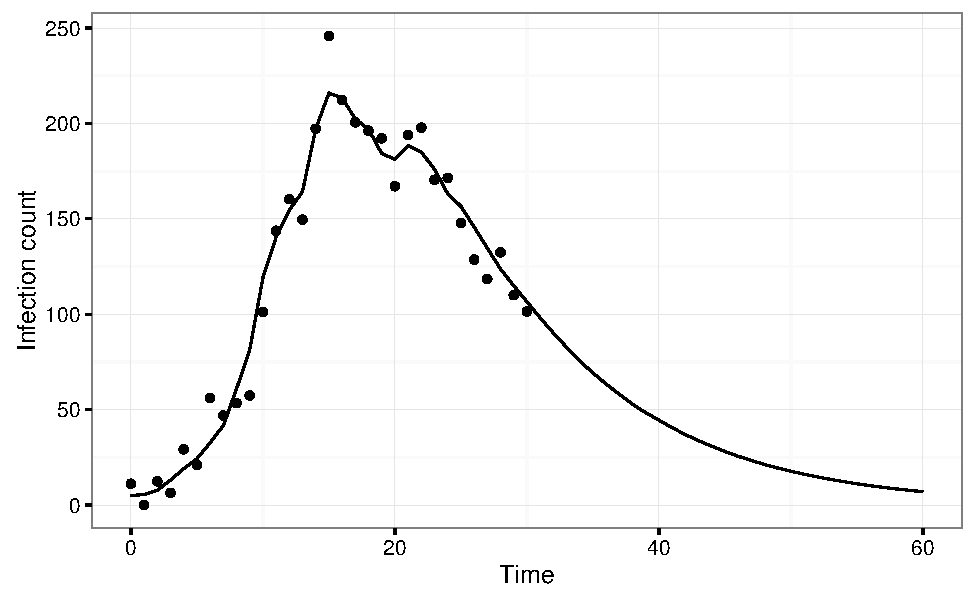
\includegraphics[width=0.8\textwidth]{./images/dataplot.pdf}
        \caption{Infection count data truncated at $T = 30$. The solid line shows the true underlying system states, and the dots show those states with added observation noise. Parameters used were $R_0 = 3.0$, $r = 0.1$, $\eta = .05$, $\sigma_{proc} = 0.5$, and additive observation noise was draw from $\mathcal{N}(0,10)$}
        \label{dataplot}
    \end{figure}

	As before, the solid line shows the true system states, while the dots show the data. In essence we want to be able to give either IF2 of HMC only the data points and have it reconstruct the entirety of the true system states.
    

\section{IF2}

	For IF2, we will take advantage of the fact that the particle filter will produce state estimates for every datum in the time series given to it, as well as producing parameter maximum likelihood point estimates. Both of these sources of information will be used to produce forecasts by parametric bootstrapping using the final parameter estimates from the particle swarm after the last IF2 pass, then using the newly generated parameter sets along with the system state point estimates from the first fitting to perform normal bootstrapping into the future of the time series.

	We will truncate the data at half the original time series length (to $T = 30$), and fit the model as previously described.

	First, we can see the state estimates for each time point produced by the last IF2 pass in Figure [\ref{if2fit}] below.

	\begin{figure}[H]
        \centering
        \captionsetup{width=.8\linewidth}
        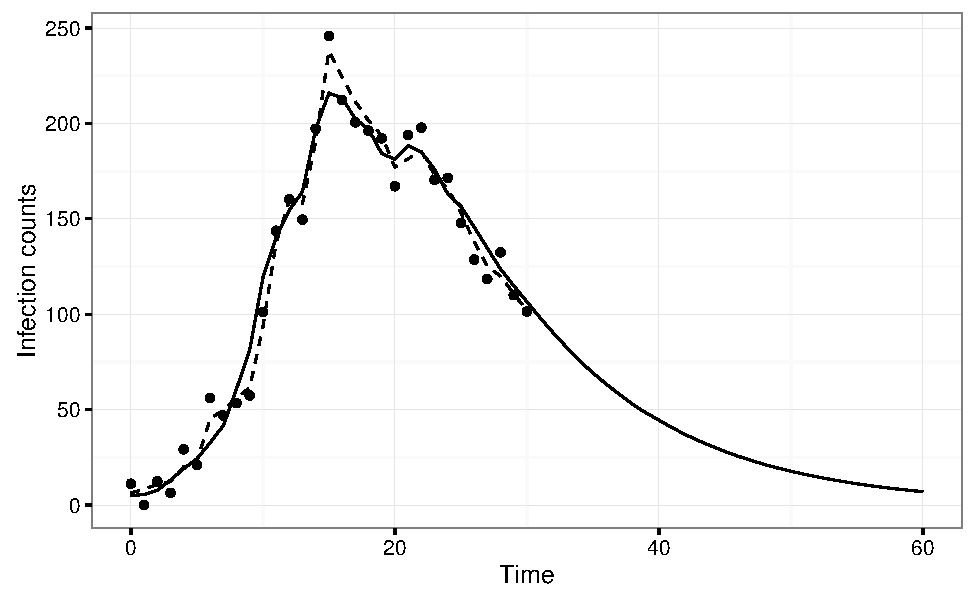
\includegraphics[width=0.8\textwidth]{./images/if2fit.pdf}
        \caption{Infection count data truncated at $T = 30$ from Figure [\ref{dataplot}] above. The dashed line shows IF2's attempt to reconstruct the true underlying state from the observed data points.}
        \label{if2fit}
    \end{figure}

    Recall that IF2 is not trying to generate parameter estimation densities, but rather produce a point estimate. Since we wish to determine the approximate distribution of each of the parameters in addition to the point estimate, we must turn to another method, parametric bootstrapping.


\subsection{Parametric Bootstrapping}

	The goal of the parametric bootstrap is use an initial density sample $\theta^*$ to generate further samples $\theta_1, \theta_2, ..., theta_M$. It works by using $\theta$ to generate artificial data sets $D_1, D_2, ..., D_M$ to which we can refit our model of interest and generate new parameter sets.

	An algorithm for parametric bootstrapping using IF2 and our stochastic SIR model is shown in Algorithm [\ref{paraboot}].

	\begin{algorithm}[H]

        \BlankLine

        \SetKwInOut{Input}{Input}
        \SetKwInOut{Output}{Output}
        \DontPrintSemicolon

        \Input{Forward simulator $S(\theta)$, data set D}

        \BlankLine

        \tcc{Initial fit}
        $\theta^* \gets IF2(D)$

        \BlankLine

        \tcc{Generate artificial data sets}
        \For{$i = 1:M$}{
	        $D_i \gets S(\theta^*)$
        }

        \BlankLine

        \tcc{Fit to new data sets}
        \For{$i = 1:M$}{
	        $\theta_i \gets IF2(D_i)$
        }

        \BlankLine

        \Output{Distribution samples $\theta_1, \theta_2, ..., \theta_M$}

        \caption{Parametric Bootstrap}\label{paraboot}

    \end{algorithm}
	

\subsection{IF2 Forecasts}

	Using the parameter sets $\theta_1, \theta_2, ..., \theta_M$ and the point estimate of the state provided by the initial IF2 fit, we can use a normal bootstrap to produce estimates of the future state. A plot showing a projection of the data from the previous plots can be seen in Figure [\ref{if2forecast}].

	\begin{figure}[H]
        \centering
        \captionsetup{width=.8\linewidth}
        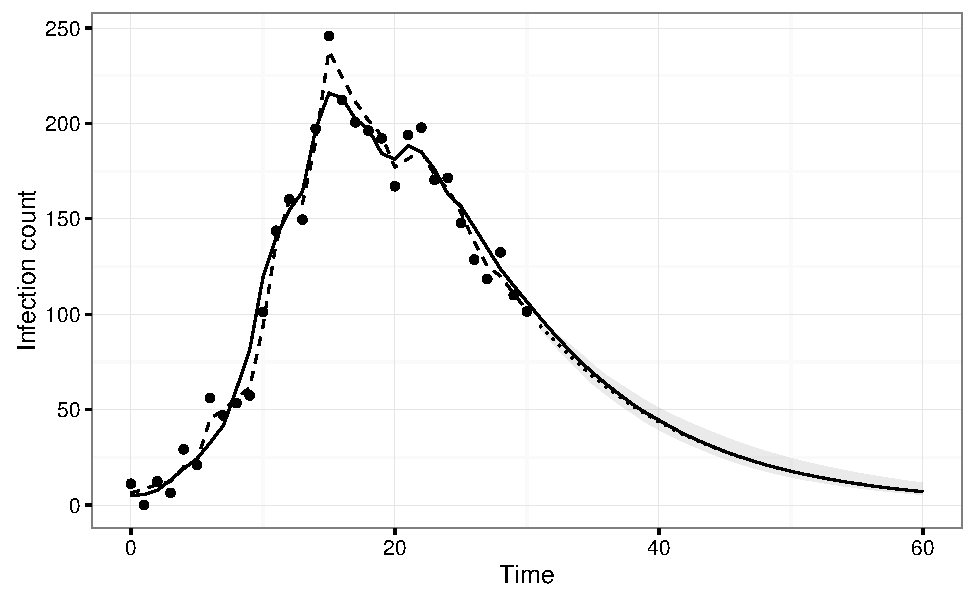
\includegraphics[width=0.8\textwidth]{./images/if2forecast.pdf}
        \caption{Forecast produced by the IF2 / parametric bootstrapping framework with $M = 200$ trajectories. The dotted line shows the mean estimate of the forecasts, and the grey ribbon shows the centre 95th quantile.}
        \label{if2forecast}
    \end{figure}

    It should be noted that the estimates produced are without added observation noise. We can see a reproduction of the data Figure [\ref{if2forecast}], but with observation noise in Figure [\ref{if2forecast_c}].

    \begin{figure}[H]
        \centering
        \captionsetup{width=.8\linewidth}
        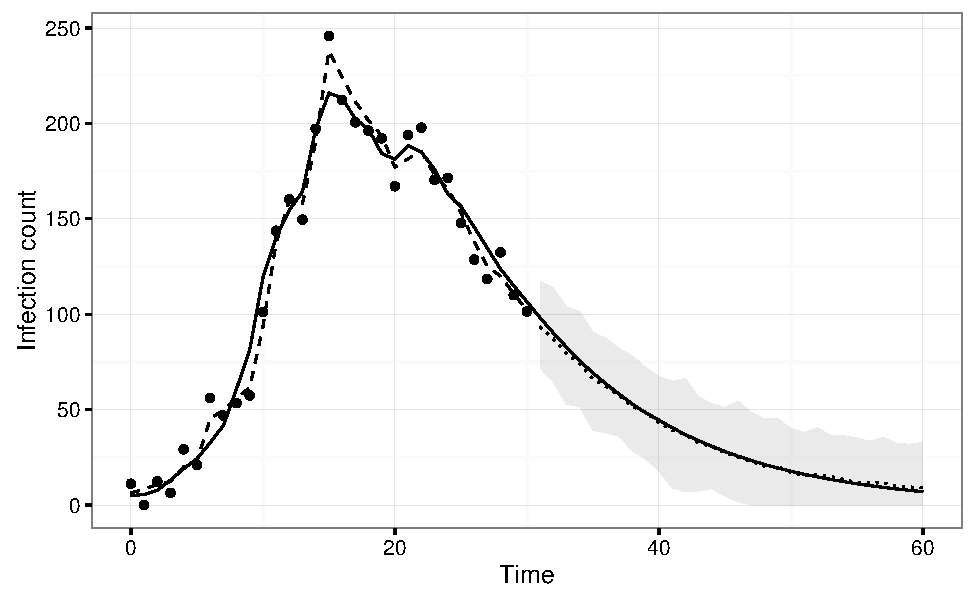
\includegraphics[width=0.8\textwidth]{./images/if2forecast_c.pdf}
        \caption{Forecast produced by the IF2 / parametric bootstrapping framework, with added observation noise drawn from the fitted parameter sets. The dotted line shows the mean estimate of the forecasts, and the grey ribbon shows the centre 95th quantile.}
        \label{if2forecast_c}
    \end{figure}

    We can define a metric to gauge forecast effectiveness by calculating the SSE and dividing that value by the number of values predicted to get the average squared error per point. For the data in Figure [\ref{if2forecast}] the value was $\overline{SSE} = 37.005$.


\section{HMCMC}

	For HMC we cannot use final state estimates as in IF2 as we only have the parameter density estimates to work with. Instead we have to rely on a pure bootstrapping approach. We are, however, not just limited to the primary parameter set samples produced by Stan -- the samples also contain estimates of the process noise present in the system, which we can use to help inform the forward simulation in portions where we have fitting data.

	As before we fit the stochastic SIR model to the partial data, but now perform bootstrapping as described above, and obtain the plot in Figure [\ref{hmcforecast}].

	\begin{figure}[H]
        \centering
        \captionsetup{width=.8\linewidth}
        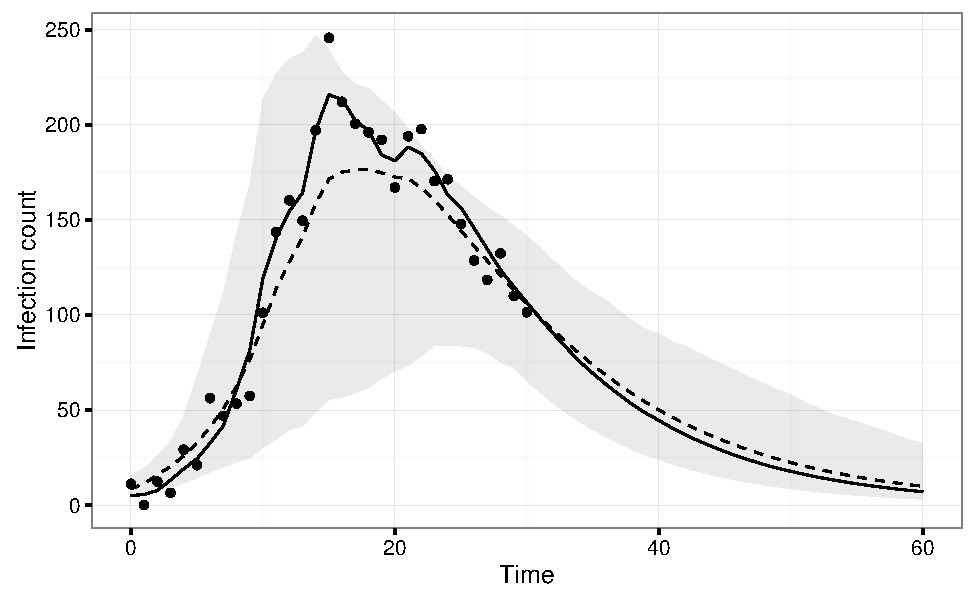
\includegraphics[width=0.8\textwidth]{./images/hmcforecast.pdf}
        \caption{Forecast produced by the HMCMC / bootstrapping framework with $M = 200$ trajectories. The dotted line shows the mean estimate of the forecasts, and the grey ribbon shows the centre 95th quantile.}
        \label{hmcforecast}
    \end{figure}

    As before we can evaluate the averaged SSE of the forecast for the data shown, giving $\overline{SSE} = 17.74223$.


\section{Truncation vs. Error}

	Of course the above mini-comparison only shows one truncation value for one trajectory. Really, we need to know how each method performs on average given different trajectories and truncation amounts. In effect we wish to ``starve'' each method of data and see how poor the estimates become with each successive data point loss.

	Using each method, we can fit the stochastic SIR model to successively smaller time series to see the effect of truncation on forecast averaged SSE. This was performed with 10 new trajectories drawn for each of the desired lengths. The results are shown in Figure [\ref{truncation}].

	\begin{figure}[H]
        \centering
        \captionsetup{width=.8\linewidth}
        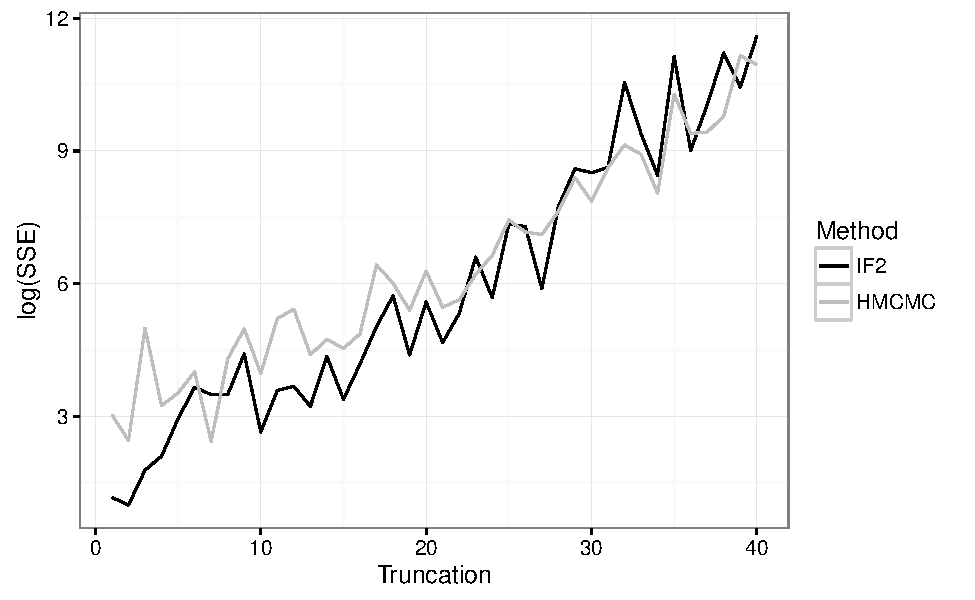
\includegraphics[width=0.8\textwidth]{./images/truncation.pdf}
        \caption{Error growth as a function of data truncation amount. Note that the y-axis shows the natural log of the averaged SSE, not the total SSE.}
        \label{truncation}
    \end{figure}

    Here we have out first real result in this paper. HMCMC consistently outperforms IF2 for truncation levels more than about 8 or 9, and does so by an increasing margin as the truncation level increases.



\end{document}